Software evolution plays an ever-increasing role in software development. Programmers rarely build software from scratch but often spend more time in modifying existing software to provide new features to customers and fix defects in existing software.  Evolving software systems is often a time-consuming and error-prone process. In fact, it is reported that 90\% of the cost of a typical software system is incurred during the maintenance phase~\cite{Madhavji2006:evolution} and a primary focus in software engineering involves issues relating to upgrading, migrating and evolving existing software systems. 

The term, {\em software evolution} dates back to 1976 when Belady and Lehman first coined this term. Software evolution refers to the {\em dynamic behavior} of software systems, as they are maintained and enhanced over their lifetimes~\cite{Belady1976:ModelEvolution}. Software evolution is particularly important as systems in organizations become longer-lived. % explain the definition of software evolution (cite: belady and lehman, etc) %L.A. Belady and M.M. Lehman, a Model of Large Program Development,o IBM Systems J., vol. 15, no. 1, pp. 225±252, 1976. 
A key notion behind this seminal work by Belady and Lehman is the concept of software system {\em entropy}. The term entropy, with a formal definition in physics relating to the amount of energy in a closed thermodynamic system is used to broadly represent a measure of the cost required to change a system or correct its natural disorder. As such, this term has had significant appeal to software engineering researchers, since it suggests a set of reasons for software maintenance. Their original work in the 1970s involved studying 20 user-oriented releases of the IBM OS/360 operating systems software, and it was the first empirical research to focus on the dynamic behavior of a relatively large and mature system (12 years old) at the time. Starting with the available data, they attempted to deduce the nature of consecutive releases of OS/360 and to postulate five {\em laws} of software evolution: (1) continuing change, (2) increasing complexity, (3) fundamental law of program evolution, (4) conservation of organizational stability, and (5) conservation of familiarity. 

Later, many researchers have systematically studied software evolution by measuring concrete metrics about software over time. 
%One of Lehman's students, Yuen studied bug data from a large operating system over time~\cite{ChongHokYuen1986:EAS}. 
Notably, Eick et al.\cite{Eick2001:CodeDecay} quantified the symptoms of {\em code decay}\textemdash {\em software is harder to change than it should be} by measuring the extent to which each risk factor matters using a rich data set of 5ESS telephone switching system. For example, they measured the number of files changed in each modification request to monitor code decay progress over time. This empirical study has influenced a variety of research projects on mining software repositories.  %The span of changes at the granularity of files increases each year.  Modularity breaks over time.  Fault potential, the likelihood of changes to induce faults increases over time.  Prediction of efforts increases over time. 

\begin{figure}[ht]
 \centering
 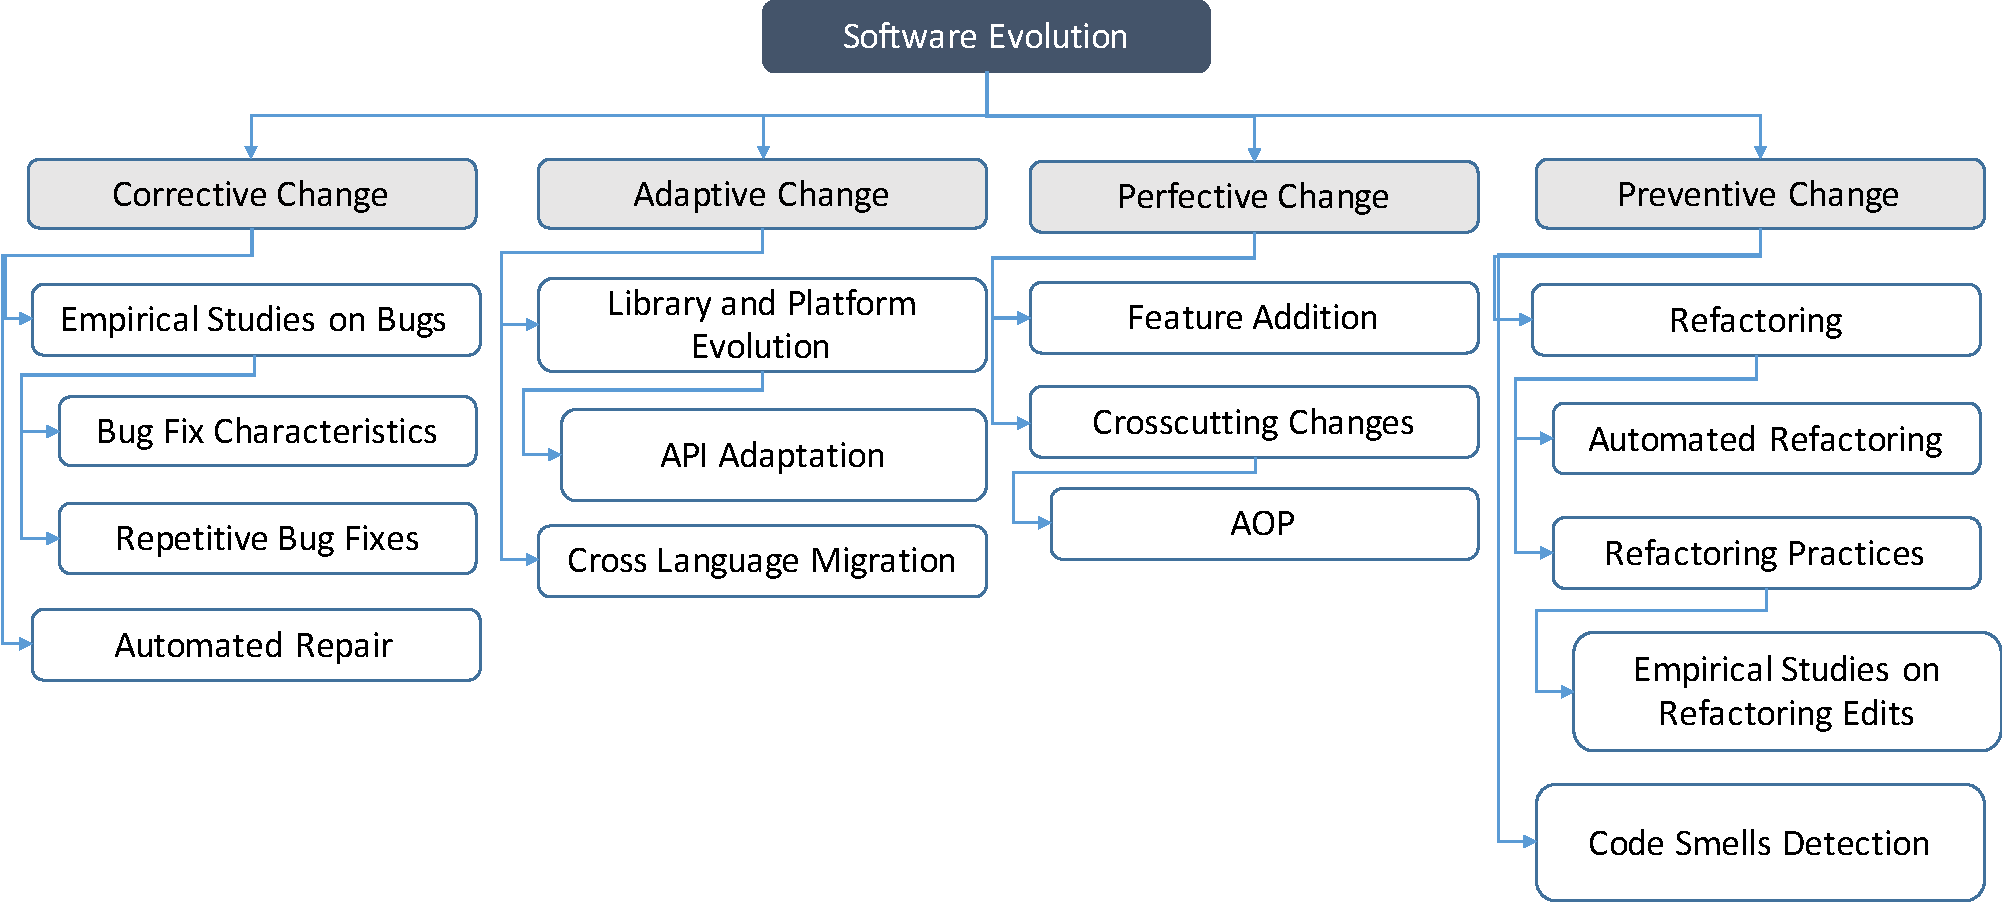
\includegraphics[width=0.95\textwidth]{images/ChangeTypesTopics.pdf}
 \caption{Change Types and Related Research Topics} 
 \label{fig:changetypetopic}
\end{figure}

Now that we accept the fact that software systems go through a {\em continuing life cycle of evolution} after the initial phase of requirement engineering, design, analysis, testing and validation, this chapter focuses an important aspect of software evolution\textemdash software changes. To that end, we first introduce the categorization of software changes into four types in Section~\ref{sec:concepts}. We then discuss the techniques of evolving software from three activity perspectives: (1) change application, (2) change inspection, and (3) change validation. In the following three sections, we provide an organized tour of seminal papers focusing on the above-mentioned three kinds of activity perspectives. 

In Section~\ref{sec:apply}, we first discuss empirical studies to summarize the characteristics of each type of software changes and then overview tool support for applying software changes. For example, for the type of {\em corrective changes}, we present several studies on the nature and extent of bug fixes. We then discuss automated techniques for fixing bugs such as automated repair. Similarly, for the type of {\em preventative changes}, we present empirical studies on refactoring practices and then discuss automated techniques for applying refactorings.  Regardless of change types, various approaches are proposed to reduce the manual effort of updated software through automation, including source-to-source program transformation, Programming by Demonstration (PbD), simultaneous editing, and systematic editing.

In Section~\ref{sec:codereview}, we overview research topics for inspecting software changes after the corresponding program modifications are made. Software engineers other than the change author often perform peer reviews by inspecting program changes, and provide feedback if they discover any suspicious software modifications. Therefore, we summarize modern code review processes and discuss techniques for examining and comprehending code changes. This section also overviews a variety of program differencing techniques that developers can use to investigate code changes and other types of techniques that raise the abstraction level of program modifications to a higher level, such as refactoring reconstruction, code change search, and evolution visualization. 

In Section~\ref{sec:debugtest}, we overview research techniques for validating software changes. 
After software modification is made, developers and testers may create new tests or reuse existing tests based on the requirements specification, run the modified software against the tests, and check whether the software executes as expected. Therefore, the activity of checking the correctness of software changes could involve failure-inducing change isolation, regression testing, and change impact analysis. 
